\begin{figure}[H]
\centering
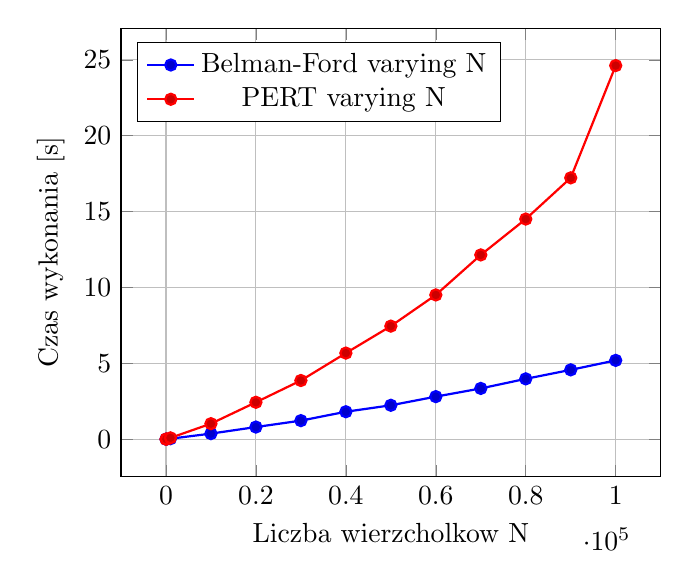
\begin{tikzpicture}
\begin{axis}[
xlabel = {Liczba wierzcholkow N},
ylabel = {Czas wykonania [s]},
legend pos = north west,
grid = both,
]
\addplot + [mark = *, thick] coordinates
    {
(10, 0.0)(100, 0.003114461898803711)(1000, 0.031162500381469727)(10000, 0.367032527923584)(20000, 0.8001964092254639)(30000, 1.2233355045318604)(40000, 1.8094770908355713)(50000, 2.2343366146087646)(60000, 2.8047921657562256)(70000, 3.345710515975952)(80000, 3.977023124694824)(90000, 4.570672512054443)(100000, 5.194704055786133)};
\addlegendentry
{Belman-Ford varying N}
\addplot + [mark = *, thick] coordinates
    {
(10, 0.001001596450805664)(100, 0.007997512817382812)(1000, 0.08727455139160156)(10000, 1.0228216648101807)(20000, 2.4322612285614014)(30000, 3.8675732612609863)(40000, 5.675054311752319)(50000, 7.453186511993408)(60000, 9.50905966758728)(70000, 12.146352767944336)(80000, 14.510110139846802)(90000, 17.22704768180847)(100000, 24.625863313674927)};
\addlegendentry
{PERT varying N}
\end{axis}
\end{tikzpicture}
\caption
{Por�wnanie czas�w wykonania algorytm�w Belman-Ford i PERT w zale�no�ci od liczby wierzcho�k�w N}
\label{fig:time_measurements_n}
\end{figure}
